\subsection{Multi-Entity Bayesian Networks}

\begin{frame}
	\begin{block}{Multi-Entity BNs~\cite{Laskey08}}
		\begin{itemize}
			\item Extends Bayesian Networks to provide first-order expressive power
			\item Extends first-order logic to provide probability distributions
			\item Support for recursion and quantifiers
			\item Built up from MEBN fragments or MFrags
			\item Every first-order sentence can be represented by an MFrag
		\end{itemize}
	\end{block}
\end{frame}

\begin{frame}
	\begin{block}{MEBN Fragment}
		An MFrag is a 5-tuple $F = ( C , I , R , G , D )$ where
		\begin{itemize}
			\item $C$ = finite set of \emph{context} value assignments
			\item $I$ = finite set of \emph{input} random variable terms
			\item $R$ = finite set of \emph{resident} random variable terms
			\item $G$ = a fragment graph
			\item $D$ = local probability distributions for each $r \in R$
		\end{itemize}
	\end{block}
\end{frame}

\begin{frame}
	\begin{figure}
		\centering
		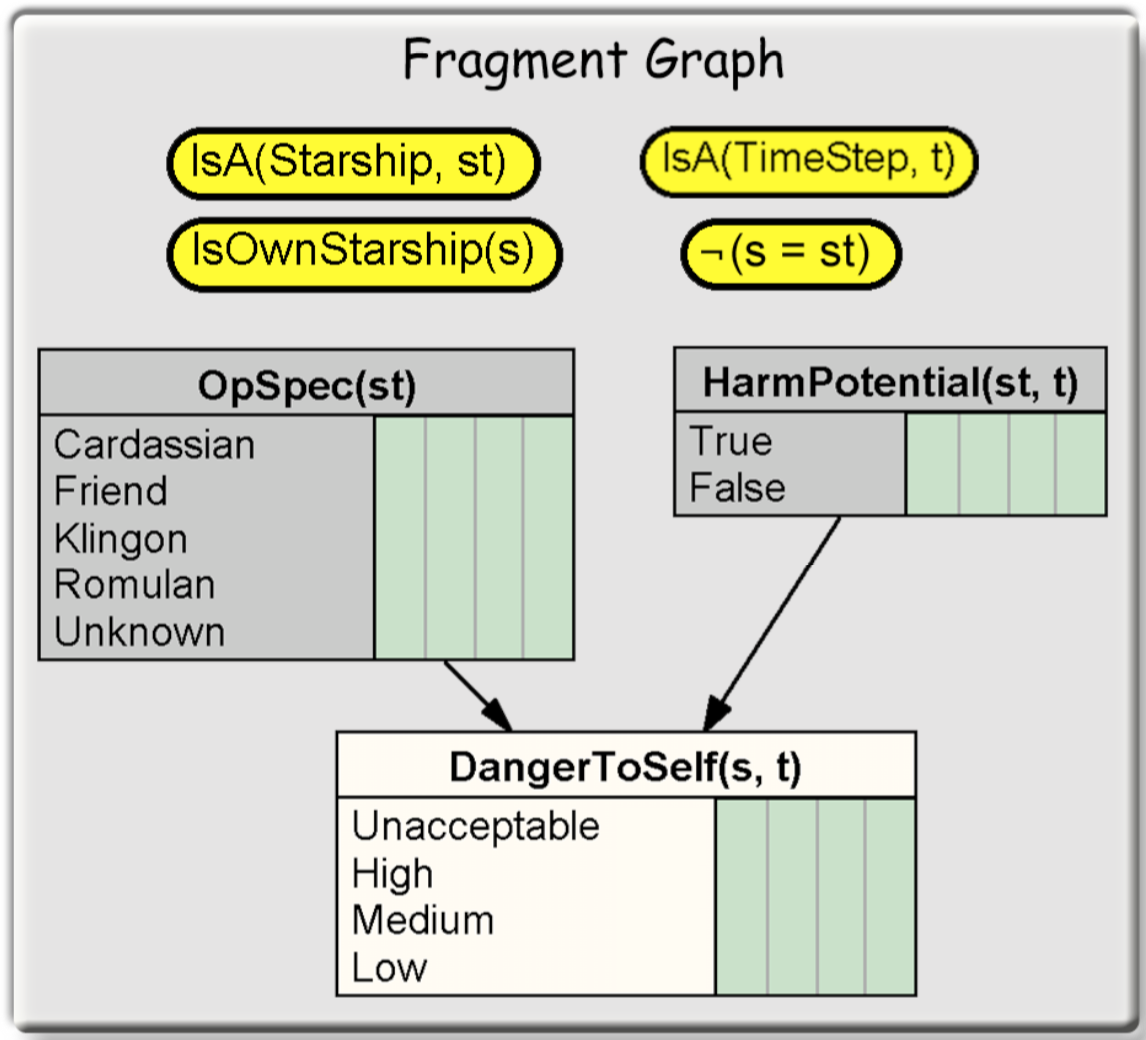
\includegraphics[height=6cm]{images/startrekmfrag}
		\caption{Danger To Self MFrag}
	\end{figure}
\end{frame}

\begin{frame}
	\begin{figure}
		\centering
		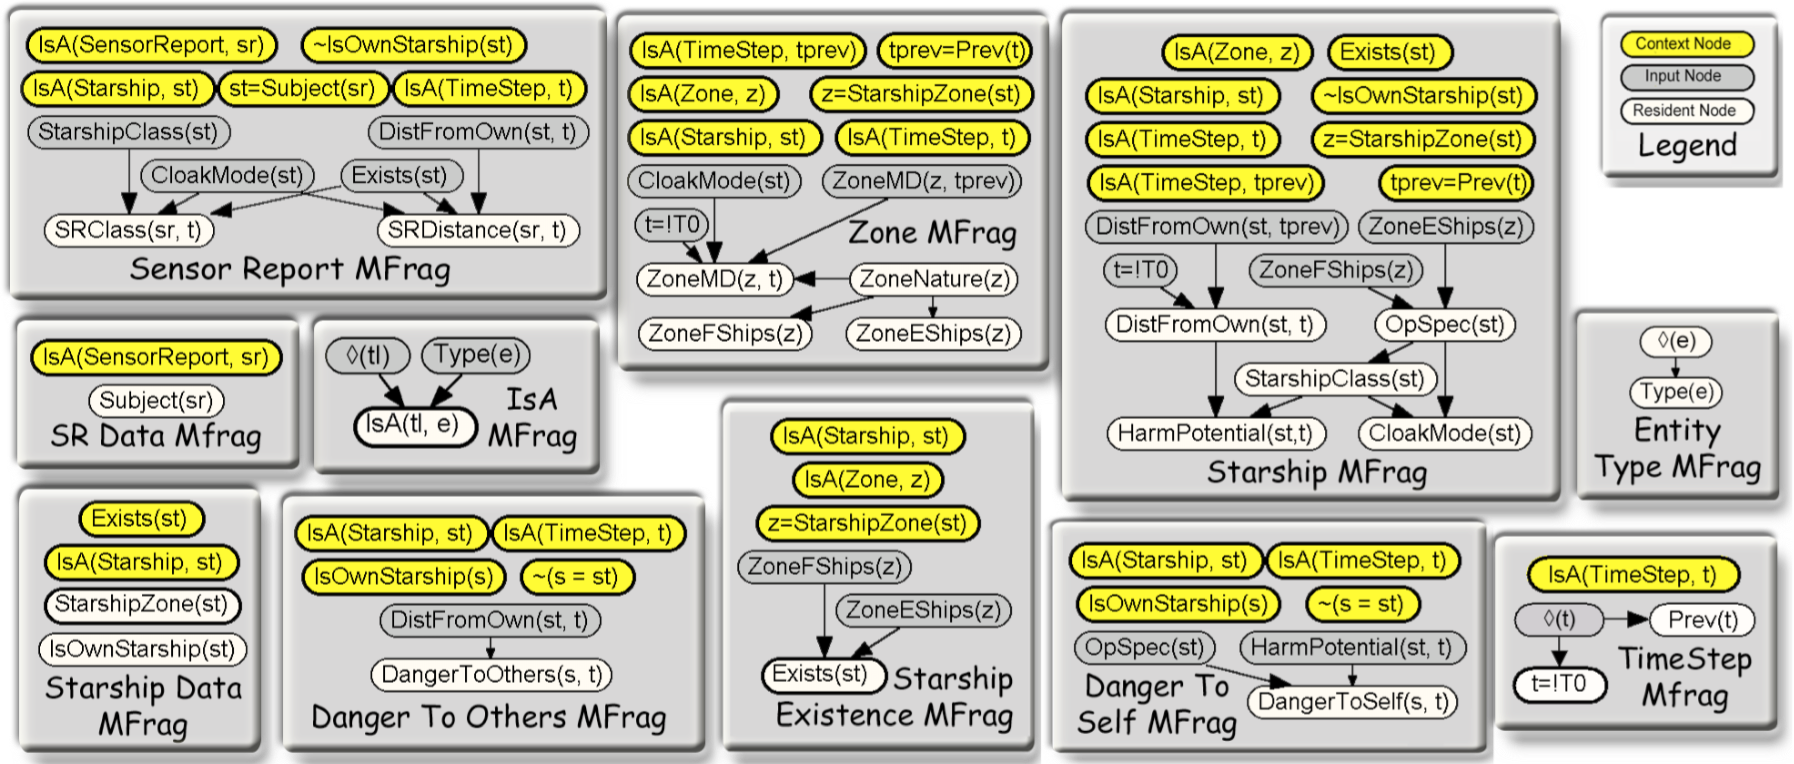
\includegraphics[width=\textwidth]{images/startrekontology}
		\caption{Star Trek MEBN}
	\end{figure}
\end{frame}